\documentclass[a4paper, 11pt]{article}

\usepackage[utf8x]{inputenc}
\usepackage[T1]{fontenc}
\usepackage{ucs}
\usepackage[english]{babel}
\usepackage{mathtools, amsmath, amsfonts}
\usepackage{fancyhdr}
\usepackage[parfill]{parskip}
\usepackage{graphicx}
\usepackage{palatino,newtxmath}
\usepackage{float}
\usepackage[font={small,it}]{caption}
\usepackage{minted}

\linespread{1.05}
\pagestyle{fancyplain}
\fancyhead{}
\fancyfoot[L]{}
\fancyfoot[C]{}
\fancyfoot[R]{\thepage}
\renewcommand{\headrulewidth}{0pt}
\renewcommand{\footrulewidth}{0pt}
\setlength{\headheight}{13.6pt}

\widowpenalty=1000
\clubpenalty=1000

\newcommand{\horrule}[1]{\rule{\linewidth}{#1}}
\def\sat{\mathbf{\;sat\;}}

\title{ 
\normalfont \normalsize 
\textsc{University of Copenhagen} \\ [25pt]
\horrule{0.5pt} \\[0.4cm]
\huge XMP: Assignment 1 \\ \Large - Programming \\
\horrule{2pt} \\[0.5cm]
}

\author{Jens Fredskov (chw752)}

\begin{document}
\maketitle
\pagebreak

\section{Implementation} % (fold)
\label{sec:implementation}

The solution has been implemented in the Go language. All source code can be found in Appendix \ref{sec:source_code}.

To run the program implementing the three problems, one must run the \texttt{main.go} main-function (this is done by running \texttt{go run main} in the source directory). This functions starts a machine for each problem (in serial order) runs it, receives its bin counts and prints these. All the components have been documented in the source code.

In general the network of communication is as in Figure \ref{fig:network}.

\begin{figure}[H]
  \centering
  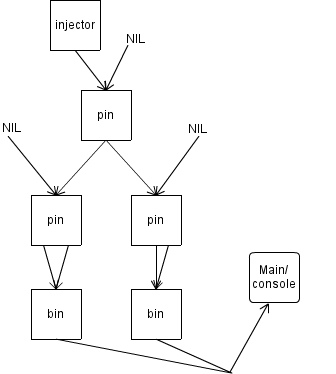
\includegraphics[width=0.6\textwidth]{network.png}
  \caption{A general overview of the communication in the implementation.}
  \label{fig:network}
\end{figure}

The injector sends the balls to a top pin, which in turn sends it to one of its ``children'' and so forth until the ball is received by a bin. This continues until the injector has sent the required number of balls. At this time the injector closes its output channel, this informs the top pin that its job is done and it will in turn close its two output channels. In general a pin closes its own output channels when both its input channels has been closed, meaning the all balls will have passed through any layers above the pin. When a bin closes it sends its ball count on a message channel which can be used e.g. for printing the bin number and ball count (as is done by the main function).

When the oscillator is added this is done by extending the pins and injector with one extra channel. The injector now always sends a message to the oscillator before it sends the ball, meaning that the skew is always up to date in the oscillator. The pins in turn send requests on a shared request channel to the oscillator. The request is done by sending the pins response channel, on which the pin will then listen, and the oscillator respond with the current skew.

% section implementation (end)

\appendix
\section{Source code} % (fold)
\label{sec:source_code}

\inputminted[fontsize=\scriptsize, frame=topline, label=machine.go, linenos=true]{go}{../src/machine.go}

\inputminted[fontsize=\scriptsize, frame=topline, label=main.go, linenos=true]{go}{../src/main.go}

% section source_code (end)

\end{document}